\documentclass[11pt,a4paper]{article}

%% ── Encodage & langue ────────────────────────────────────────
\usepackage[utf8]{inputenc}
\usepackage[T1]{fontenc}
\usepackage[french]{babel}

%% ── Mise en page ─────────────────────────────────────────────
\usepackage{geometry}
\geometry{top=2.5cm, bottom=2.8cm, left=2.8cm, right=2.8cm}
\usepackage{lmodern}
\usepackage{microtype}
\usepackage{parskip}
\setlength{\parskip}{6pt}
\setlength{\parindent}{0pt}

%% ── Couleurs ─────────────────────────────────────────────────
\usepackage{xcolor}
\definecolor{hecDark}{RGB}{31,56,100}
\definecolor{hecBlue}{RGB}{46,84,150}
\definecolor{hecGray}{RGB}{89,89,89}
\definecolor{rowHead}{RGB}{217,225,242}
\definecolor{rowAlt}{RGB}{242,245,250}
\definecolor{rowGreen}{RGB}{226,239,218}

%% ── Tableaux ─────────────────────────────────────────────────
\usepackage{booktabs}
\usepackage{array}
\usepackage{tabularx}
\usepackage{longtable}
\usepackage{colortbl}
\usepackage{multirow}
\renewcommand{\arraystretch}{1.35}
\newcolumntype{L}[1]{>{\raggedright\arraybackslash}p{#1}}
\newcolumntype{C}[1]{>{\centering\arraybackslash}p{#1}}
\newcolumntype{R}[1]{>{\raggedleft\arraybackslash}p{#1}}
\newcolumntype{X}{>{\raggedright\arraybackslash}X}

%% ── Maths ────────────────────────────────────────────────────
\usepackage{amsmath}
\usepackage{amssymb}

%% ── En-têtes & pieds ─────────────────────────────────────────
\usepackage{fancyhdr}
\pagestyle{fancy}
\fancyhf{}
\fancyhead[L]{\small\color{hecGray}Techniques d'exploitation de données (60600)}
\fancyhead[R]{\small\color{hecGray}HEC Montréal -- Hiver 2026}
\fancyfoot[C]{\small\color{hecGray}\thepage}
\renewcommand{\headrulewidth}{0.4pt}
\renewcommand{\footrulewidth}{0pt}

%% ── Titres ───────────────────────────────────────────────────
\usepackage{titlesec}
\titleformat{\section}
  {\large\bfseries\color{hecDark}}{\thesection}{0.8em}{}[\vspace{-4pt}\rule{\linewidth}{0.6pt}\vspace{2pt}]
\titleformat{\subsection}
  {\normalsize\bfseries\color{hecBlue}}{\thesubsection}{0.8em}{}
\titleformat{\subsubsection}
  {\normalsize\itshape\bfseries\color{hecBlue}}{\thesubsubsection}{0.8em}{}
\titlespacing{\section}{0pt}{14pt}{6pt}
\titlespacing{\subsection}{0pt}{10pt}{4pt}
\titlespacing{\subsubsection}{0pt}{8pt}{3pt}

%% ── Listes ───────────────────────────────────────────────────
\usepackage{enumitem}
\setlist[itemize]{noitemsep, topsep=3pt, leftmargin=1.4em}

%% ── Références ───────────────────────────────────────────────
\usepackage[
  backend=biber,
  style=apa,
  sorting=nyt,
  maxbibnames=9
]{biblatex}
\addbibresource{references.bib}

%% ── Hyperliens ───────────────────────────────────────────────
\usepackage{hyperref}
\hypersetup{
  colorlinks=true,
  linkcolor=hecBlue,
  urlcolor=hecBlue,
  citecolor=hecBlue,
  pdftitle={Travail en équipe -- MATH60600 -- HEC Montréal},
  pdfauthor={Youssouf A. et Marc B.}
}

%% ── Utilitaires ──────────────────────────────────────────────
\usepackage{caption}
\captionsetup[table]{
  labelfont={bf,color=hecDark},
  textfont={small},
  skip=4pt,
  position=top
}
\usepackage{float}
\usepackage{graphicx}

%% ── Raccourcis ───────────────────────────────────────────────
\newcommand{\hdr}[1]{\cellcolor{rowHead}\textbf{#1}}
\newcommand{\hlg}[1]{\cellcolor{rowGreen}#1}
\newcommand{\code}[1]{\texttt{\small #1}}

% ─────────────────────────────────────────────────────────────
\begin{document}

%% ════════════════════════════════════════════════════════════
%% PAGE DE TITRE
%% ════════════════════════════════════════════════════════════
\begin{titlepage}
\centering
\vspace*{0.8cm}


\includegraphics[width=3.5cm]{logo_hec.png}

\vspace{0.6cm}
{\color{hecDark}\rule{\linewidth}{1.5pt}}
\vspace{0.4cm}

{\LARGE\bfseries\color{hecDark} Travail en équipe\par}
\vspace{0.35cm}
{\large\bfseries\color{hecBlue}
  Techniques d'exploitation de données (MATH60600)\par}
\vspace{0.2cm}
{\normalsize Classification multi-classes et optimisation d'hyperparamètres\par
 pour des données de jeux mobiles\par}

\vspace{0.3cm}
{\color{hecDark}\rule{\linewidth}{0.8pt}}

\vspace{1.2cm}
{\normalsize
  \textbf{Professeurs :} Denis Larocque et Mina Arzaghi \quad
  \textbf{Remise :} 31 mars 2026\par}

\vspace{1.4cm}

\begin{tabular}{L{4.5cm} C{3.2cm} L{5cm}}
\toprule
\rowcolor{rowHead}
\textbf{Membre} & \textbf{Matricule} & \textbf{Programme} \\
\midrule
Youssouf A. & -- & M.Sc. Intelligence d'affaires \\
Marc B.     & -- & M.Sc. Intelligence d'affaires \\
\bottomrule
\end{tabular}

\vspace{1.5cm}
{\normalsize\textbf{Compétition Kaggle :}
  \url{https://www.kaggle.com/t/b44be49a21aa4f319b88b82c261d5a08}\par}

\vspace{0.6cm}
{\normalsize\textbf{Score Kaggle Public :}
  \textbf{\color{hecDark}0.849} -- 2\textsuperscript{e} au classement\par}

\vfill
{\small\color{hecGray} HEC Montréal -- Hiver 2026}
\end{titlepage}

\newpage
\setcounter{page}{1}

%% ════════════════════════════════════════════════════════════
\section{Introduction}
%% ════════════════════════════════════════════════════════════

Ce rapport présente les travaux réalisés dans le cadre du travail en équipe
du cours \textbf{Techniques d'exploitation de données (MATH60600)}, autour
de deux problématiques issues de l'industrie des jeux mobiles.

La \textbf{Partie~A} porte sur un problème de classification multi-classes
($Y \in \{1,2,3,4\}$) visant à prédire quel jeu un joueur installera en
premier. Nous développons une architecture de stacking à trois niveaux
intégrant les approches One-vs-One (OvO) et One-vs-All (OvA)
\parencite{galar2011}, le méta-modèle de Wolpert (\citeyear{wolpert1992})
et Breiman (\citeyear{breiman1996}), et la technique de seed averaging
issue de \textcite{izmailov2018}. Notre meilleure soumission atteint
\textbf{0.849 sur le tableau public Kaggle} (2\textsuperscript{e} sur 6
soumissions).

La \textbf{Partie~B} traite de la prédiction de la Customer Lifetime Value
(CLV). Nous comparons trois méthodes d'optimisation des hyperparamètres :
Grid Search, Random Search \parencite{bergstra2012}, et optimisation
bayésienne via Optuna/TPE \parencite{akiba2019}.

%% ════════════════════════════════════════════════════════════
\section{Données et prétraitement}
%% ════════════════════════════════════════════════════════════

\subsection{Données -- Partie A (classification)}

La Partie~A s'appuie sur \code{train.csv} (5\,000 observations, 17 variables)
et \code{test.csv} (55\,000 observations). Les quatre classes de $Y$ sont
quasi-équilibrées (24,7\,\% à 25,9\,\%), ce qui justifie l'accuracy comme
métrique principale.

\subsection{Feature engineering -- Partie A}

Treize ratios comportementaux ont été construits à partir des 16 variables
originales, auxquels s'ajoutent des transformations logarithmiques/racine,
des interactions, un target encoding et un clustering K-Means ($k=5$), pour
un total de \textbf{58 variables explicatives}.

\begin{table}[H]
\caption{Variables dérivées créées lors du feature engineering}
\label{tab:fe}
\centering\small
\begin{tabularx}{\linewidth}{L{4.2cm} L{4.6cm} X}
\toprule
\rowcolor{rowHead}
\textbf{Variable} & \textbf{Formule} & \textbf{Justification} \\
\midrule
\code{avg\_purchase\_value}       & \code{totpurchases / (numpurchases+1)}  & Valeur monétaire moyenne par achat \\
\rowcolor{rowAlt}
\code{avg\_playtime\_per\_session}& \code{totplaytime / (numsessions+1)}    & Durée moyenne d'engagement par session \\
\code{avg\_playtime\_per\_day}    & \code{totplaytime / (numdays+1)}        & Intensité de jeu journalière \\
\rowcolor{rowAlt}
\code{purchases\_per\_day}        & \code{numpurchases / (numdays+1)}       & Fréquence d'achat journalière \\
\code{sessions\_per\_day}         & \code{numsessions / (numdays+1)}        & Fréquence de connexion journalière \\
\rowcolor{rowAlt}
\code{score\_per\_life}           & \code{totscore / (numlives+1)}          & Efficacité relative du joueur \\
\code{elements\_per\_day}         & \code{numelements / (numdays+1)}        & Richesse de l'expérience journalière \\
\rowcolor{rowAlt}
\code{skill\_combined/diff/sum}   & \code{skill1*skill2}, différence, somme & Interactions entre compétences \\
\code{trend\_combined}            & \code{trendsession + trendpurchase}     & Signal de tendance agrégé \\
\rowcolor{rowAlt}
\code{trend\_intensity}           & \code{trendpurchase * totpurchases}     & Signal d'achat pondéré par le volume \\
\code{engagement\_rate}           & \code{numdays / 7.0}                    & Taux de présence sur la semaine \\
\rowcolor{rowAlt}
\code{purchase\_intensity}        & \code{numpurchases / (totplaytime+1)}   & Propension à acheter par heure jouée \\
\code{log\_ / sqrt\_ (5 cols)}    & \code{log1p} et \code{sqrt} sur 5 variables & Réduction de l'asymétrie des distributions \\
\bottomrule
\end{tabularx}
\end{table}

En complément, 8 variables de target encoding (\code{country} et
\code{difflevel} $\times$ 4 classes) et 1 variable de clustering K-Means
ont été ajoutées. Le clustering est fitté exclusivement sur le train pour
éviter tout data leakage.

\subsection{Données CLV -- Partie B}

La Partie~B utilise \code{clv\_mobile\_data\_train.txt} et
\code{clv\_mobile\_data\_test.txt} (5\,000 obs. chacun, 17 variables).
La variable cible $Y$ est continue ($\min=10.46$, $\max=106.72$,
$\bar{Y}=30.69$). Toutes les variables du fichier sont numériques.

%% ════════════════════════════════════════════════════════════
\section{Partie A -- Classification multi-classes}
%% ════════════════════════════════════════════════════════════

\subsection{Protocole de validation}

L'ensemble des modèles est évalué par \textbf{validation croisée OOF
(Out-Of-Fold) stratifiée à 5 folds} sur les 5\,000 observations
d'entraînement. Chaque observation est prédite uniquement par des modèles
entraînés sur les folds ne la contenant pas, ce qui élimine tout risque de
data leakage dans le stacking \parencite{wolpert1992, breiman1996}.

\subsection{Approche OvO et OvA -- \textcite{galar2011}}

Conformément à l'exigence du cours, nous implémentons les deux
décompositions binaires du problème multi-classes décrites par
\textcite{galar2011}.

\begin{itemize}
  \item \textbf{One-vs-One (OvO) :} entraîne $\binom{4}{2} = 6$
    classifieurs binaires, chacun distinguant une paire de classes $(i,j)$.
    Les probabilités sont obtenues via \code{decision\_function()} suivi
    d'une normalisation softmax.
  \item \textbf{One-vs-All (OvA) :} entraîne $K=4$ classifieurs
    indépendants, chacun opposant une classe à toutes les autres.
\end{itemize}

Les hyperparamètres de l'OvO ont été optimisés par Random Search (30
itérations $\times$ 3 folds) conformément à \textcite{bergstra2012},
aboutissant aux paramètres retenus :
\code{n\_estimators=413}, \code{max\_depth=3}, \code{learning\_rate=0.199}.
L'évaluation isolée CV-5 confirme la supériorité de OvO :

\begin{table}[H]
\caption{Comparaison OvO vs OvA en validation croisée CV-5 isolée
         \parencite{galar2011}}
\label{tab:ovo_ova}
\centering\small
\begin{tabular}{L{5.5cm} C{2.5cm} C{2.5cm} C{3cm}}
\toprule
\rowcolor{rowHead}
\textbf{Modèle} & \textbf{CV-5 moyen} & \textbf{Écart-type} & \textbf{Gain vs OvA} \\
\midrule
OvA GBM (défaut)       & 0.7446 & $\pm$0.0185 & -- \\
\rowcolor{rowGreen}
OvO GBM (optimisé RS)  & 0.8064 & $\pm$0.0121 & \textbf{+0.0618} \\
\bottomrule
\end{tabular}
\end{table}

Les deux approches sont ensuite intégrées comme modèles de Niveau~1 dans
le pipeline de stacking.

\subsection{Architecture du stacking 3 niveaux}

Le modèle final repose sur un stacking à 3 niveaux
\parencite{wolpert1992, breiman1996}.

\begin{table}[H]
\caption{Architecture du stacking 3 niveaux}
\label{tab:stacking}
\centering\small
\begin{tabularx}{\linewidth}{C{1.8cm} L{5.5cm} X}
\toprule
\rowcolor{rowHead}
\textbf{Niveau} & \textbf{Modèles} & \textbf{Sortie OOF} \\
\midrule
\textbf{1} &
  XGBoost, LightGBM, OvA GBM, OvO GBM \parencite{galar2011},
  CatBoost \parencite{prokhorenkova2018}, AdaBoost &
  24 colonnes (6 modèles $\times$ 4 classes) \\
\rowcolor{rowAlt}
\textbf{2} &
  L2\_XGBoost, L2\_LightGBM, L2\_CatBoost &
  12 colonnes (3 modèles $\times$ 4 classes) \\
\textbf{3} &
  Méta-modèle XGBoost final &
  12 OOF L2 + 69 features prétraitées = 81 colonnes \\
\bottomrule
\end{tabularx}
\end{table}

L'ajout des features originales prétraitées au méta-modèle de Niveau~3
(81 colonnes au lieu de 12) apporte un gain mesuré de \textbf{+0.010
d'accuracy CV}.

\subsection{Seed Averaging}

Pour réduire la variance stochastique, le pipeline complet est entraîné
5 fois avec des seeds distincts (42, 0, 123, 777, 2024), puis les
probabilités de prédiction sont moyennées avant l'argmax final. Cette
technique s'inscrit dans le prolongement de deux travaux :

\begin{itemize}
  \item \textcite{izmailov2018} démontrent que l'averaging de plusieurs
    solutions stochastiques conduit à des optima plus plats de la surface
    de perte, avec une meilleure généralisation que les solutions issues
    d'un seul entraînement.
  \item \textcite{zhou2025} confirment qu'une variance significative de
    performance est observable selon le choix du seed, et recommandent
    l'averaging multi-seeds pour stabiliser l'inférence.
\end{itemize}

Conformément à ces recommandations, cette technique a apporté un gain
empirique de \textbf{+0.008 sur le score Kaggle Public} (v8 $\to$ v9).

\subsection{Résultats}

\subsubsection{Progression itérative v1 à v9}

\begin{table}[H]
\caption{Progression itérative de la solution}
\label{tab:progression}
\centering\small
\begin{tabularx}{\linewidth}{C{1.3cm} X C{2cm} C{2.4cm}}
\toprule
\rowcolor{rowHead}
\textbf{Version} & \textbf{Amélioration apportée} & \textbf{CV OOF} & \textbf{Kaggle Public} \\
\midrule
v1 & Baseline XGBoost (défaut) & -- & 0.781 \\
\rowcolor{rowAlt}
v2 & Correction variables catégorielles & -- & 0.786 \\
v3/v4 & Feature engineering (13 vars) + OvO/OvA \parencite{galar2011} & -- & 0.788 \\
\rowcolor{rowAlt}
v5 & Stacking OOF LR (5 modèles) \parencite{wolpert1992} & 0.8064 & 0.826 \\
v6 & Stacking XGBoost méta + OvO optimisé \parencite{bergstra2012} & 0.8224 & 0.834 \\
\rowcolor{rowAlt}
v7 & Stacking 2 niveaux + features originales dans méta & 0.8246 & 0.840 \\
v8 & Ajout AdaBoost (6 modèles N1) \parencite{prokhorenkova2018} & 0.8258 & 0.841 \\
\rowcolor{rowGreen}
\textbf{v9} & \textbf{Seed averaging 5 seeds \parencite{izmailov2018,zhou2025} -- RETENU} & \textbf{0.8281} & \textbf{0.849} \\
\bottomrule
\end{tabularx}
\end{table}

\subsubsection{Résultats CV par seed (v9)}

\begin{table}[H]
\caption{Scores CV par seed -- pipeline v9}
\label{tab:seeds}
\centering\small
\begin{tabular}{C{2.2cm} C{2.8cm} C{2.8cm} L{5.5cm}}
\toprule
\rowcolor{rowHead}
\textbf{Seed} & \textbf{CV-5 moyen} & \textbf{Écart-type} & \textbf{Note} \\
\midrule
42   & 0.8294 & $\pm$0.0062 & \\
\rowcolor{rowAlt}
0    & 0.8290 & $\pm$0.0085 & \\
123  & 0.8296 & $\pm$0.0096 & Meilleur seed individuel \\
\rowcolor{rowAlt}
777  & 0.8236 & $\pm$0.0098 & \\
2024 & 0.8288 & $\pm$0.0122 & \\
\midrule
\rowcolor{rowGreen}
\textbf{Moyenne} & \textbf{0.8281} & \textbf{$\pm$0.0023} &
  Kaggle Public : \textbf{0.849} \\
\bottomrule
\end{tabular}
\end{table}

\subsubsection{Classement Kaggle Public}

\begin{table}[H]
\caption{Classement Kaggle Public (9\,\% des données test)}
\label{tab:kaggle}
\centering\small
\begin{tabular}{C{1.5cm} L{5.5cm} C{2.8cm} C{2.5cm}}
\toprule
\rowcolor{rowHead}
\textbf{Rang} & \textbf{Équipe} & \textbf{Score Public} & \textbf{Soumissions} \\
\midrule
1 & yanziyang & 0.851 & 16 \\
\rowcolor{rowGreen}
\textbf{2} & \textbf{Youssouf A. et Marc B.} & \textbf{0.849} & \textbf{6} \\
\bottomrule
\end{tabular}
\end{table}

\textbf{Note sur le risque d'overfitting Public/Private LB :} le score
Public LB est calculé sur 9\,\% du test ($\approx$4\,950 obs.), tandis
que le Private LB (91\,\%) détermine le classement final. Toute
l'optimisation a été conduite sur le CV interne du train set, jamais sur
les données test, ce qui minimise le risque d'overfitting au Public LB
\parencite{bergstra2012}.

%% ════════════════════════════════════════════════════════════
\section{Partie B -- Optimisation des hyperparamètres}
%% ════════════════════════════════════════════════════════════

\subsection{Ressources identifiées}

\begin{table}[H]
\caption{Ressources identifiées pour l'optimisation des hyperparamètres}
\label{tab:ressources}
\centering\small
\begin{tabularx}{\linewidth}{L{3.2cm} X L{4.5cm}}
\toprule
\rowcolor{rowHead}
\textbf{Ressource} & \textbf{Contenu et pertinence} & \textbf{Référence} \\
\midrule
Article fondateur &
  Démontre formellement que Random Search surpasse Grid Search lorsque
  certains hyperparamètres ont peu d'influence. Fondement de notre
  choix de Random Search et de l'optimisation OvO en Partie~A. &
  \textcite{bergstra2012} \\
\rowcolor{rowAlt}
Manuel pédagogique &
  Décrit l'implémentation pratique de \code{GridSearchCV} et
  \code{RandomizedSearchCV} avec scikit-learn. Recommandations sur les
  espaces de recherche et la validation croisée imbriquée sans leakage. &
  \textcite{geron2019} \\
Framework bayésien &
  Présente l'algorithme TPE (Tree-structured Parzen Estimator) qui
  guide la recherche en exploitant l'historique via un modèle surrogate.
  Troisième génération après Grid Search et Random Search. &
  \textcite{akiba2019} \\
\bottomrule
\end{tabularx}
\end{table}

\subsection{Description des trois méthodes}

\subsubsection{Grid Search}

\textbf{Principe :} teste exhaustivement toutes les combinaisons d'une
grille discrète. Pour $k$ hyperparamètres avec $n_1, \ldots, n_k$ valeurs,
le nombre d'évaluations est $n_1 \times \cdots \times n_k \times F$
\parencite{geron2019}.

\textbf{Avantages/limites :} déterministe, garantit l'optimum dans la
grille définie. Coût exponentiel; ne peut pas explorer de valeurs continues
entre les points de grille.

\subsubsection{Random Search}

\textbf{Principe :} tire aléatoirement $n$ configurations depuis des
distributions continues \parencite{bergstra2012}. Surpasse Grid Search
quand seuls quelques hyperparamètres sont réellement influents car la
probabilité d'en couvrir au moins un est plus élevée.

\textbf{Avantages/limites :} explore un espace continu plus large avec un
budget fixe. Non déterministe, n'exploite pas l'historique des évaluations.

\subsubsection{Optimisation bayésienne (Optuna/TPE)}

\textbf{Principe :} construit un modèle probabiliste (surrogate) de la
fonction $f(\text{hyperparamètres}) \to \text{performance}$. À chaque
itération, maximise l'Expected Improvement pour choisir le prochain point
\parencite{akiba2019}.

\textbf{Avantages/limites :} converge plus rapidement grâce au guidage par
l'historique. Overhead du modèle surrogate; moins facilement
parallélisable.

\subsection{Application sur CLV -- RandomForestRegressor}

Les trois méthodes sont appliquées au même modèle avec le même budget :
50 configurations $\times$ 5 folds = 250 évaluations (135 pour Grid
Search). Trois hyperparamètres sont optimisés :
\code{n\_estimators} $\in [100, 800]$,
\code{max\_features} $\in [0.1, 1.0]$,
\code{min\_samples\_leaf} $\in [1, 20]$.

\subsection{Résultats}

\begin{table}[H]
\caption{Comparaison des méthodes d'optimisation -- RandomForestRegressor}
\label{tab:partieB}
\centering\small
\begin{tabularx}{\linewidth}{L{3.2cm} C{2cm} C{2.2cm} C{2.2cm} X}
\toprule
\rowcolor{rowHead}
\textbf{Méthode} & \textbf{R$^2$ CV-5} & \textbf{Gain} &
  \textbf{Évaluations} & \textbf{Meilleurs paramètres} \\
\midrule
Baseline (défaut) & 0.7665 & -- & -- &
  \code{n\_est=500} \\
\rowcolor{rowAlt}
Grid Search \parencite{geron2019} & 0.7694 & +0.0029 & 135 (27$\times$5) &
  \code{max\_feat=0.5, n=500, leaf=1} \\
Random Search \parencite{bergstra2012} & 0.7721 & +0.0056 & 250 (50$\times$5) &
  \code{max\_feat=0.696, n=489, leaf=2} \\
\rowcolor{rowGreen}
\textbf{Optuna/TPE} \parencite{akiba2019} & \textbf{0.7719} & +0.0054 &
  250 (50$\times$5) &
  \code{max\_feat=0.662, n=753, leaf=1} \\
\bottomrule
\multicolumn{5}{l}{\small Modèle final (test 20\,\%) :
  $R^2 = 0.7933$, RMSE $= 5.5843$, MAE $= 4.2406$}
\end{tabularx}
\end{table}

Les résultats confirment \textcite{bergstra2012} : Random Search et Optuna
identifient des valeurs continues de \code{max\_features} (0.696 et 0.662)
inaccessibles à une grille discrète, ce qui explique leur avantage. La
convergence d'Optuna est plus rapide -- le meilleur résultat est trouvé
dans les 15 premiers trials -- confirmant l'efficacité du modèle surrogate
décrit par \textcite{akiba2019}.

\subsection{Visualisations}

\begin{figure}[H]
  \centering
  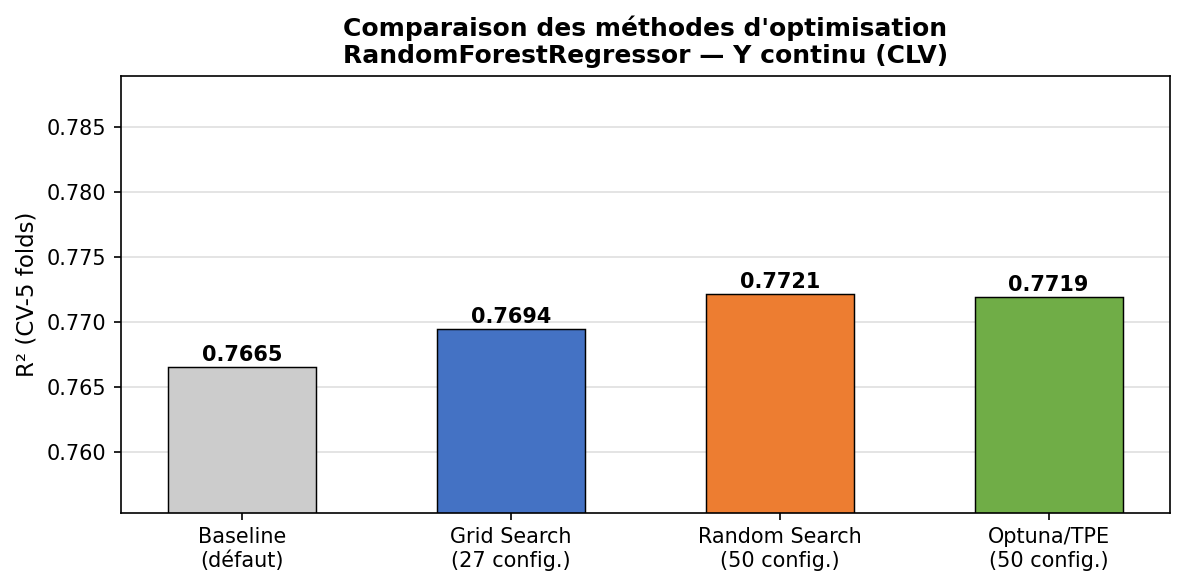
\includegraphics[width=\linewidth]{graph_comparaison_methodes.png}
  \caption{Comparaison des $R^2$ (CV-5) selon la méthode d'optimisation.
           Random Search \parencite{bergstra2012} et Optuna/TPE
           \parencite{akiba2019} surpassent le Grid Search grâce à
           l'exploration continue de l'espace des hyperparamètres.}
  \label{fig:comparaison}
\end{figure}

\begin{figure}[H]
  \centering
  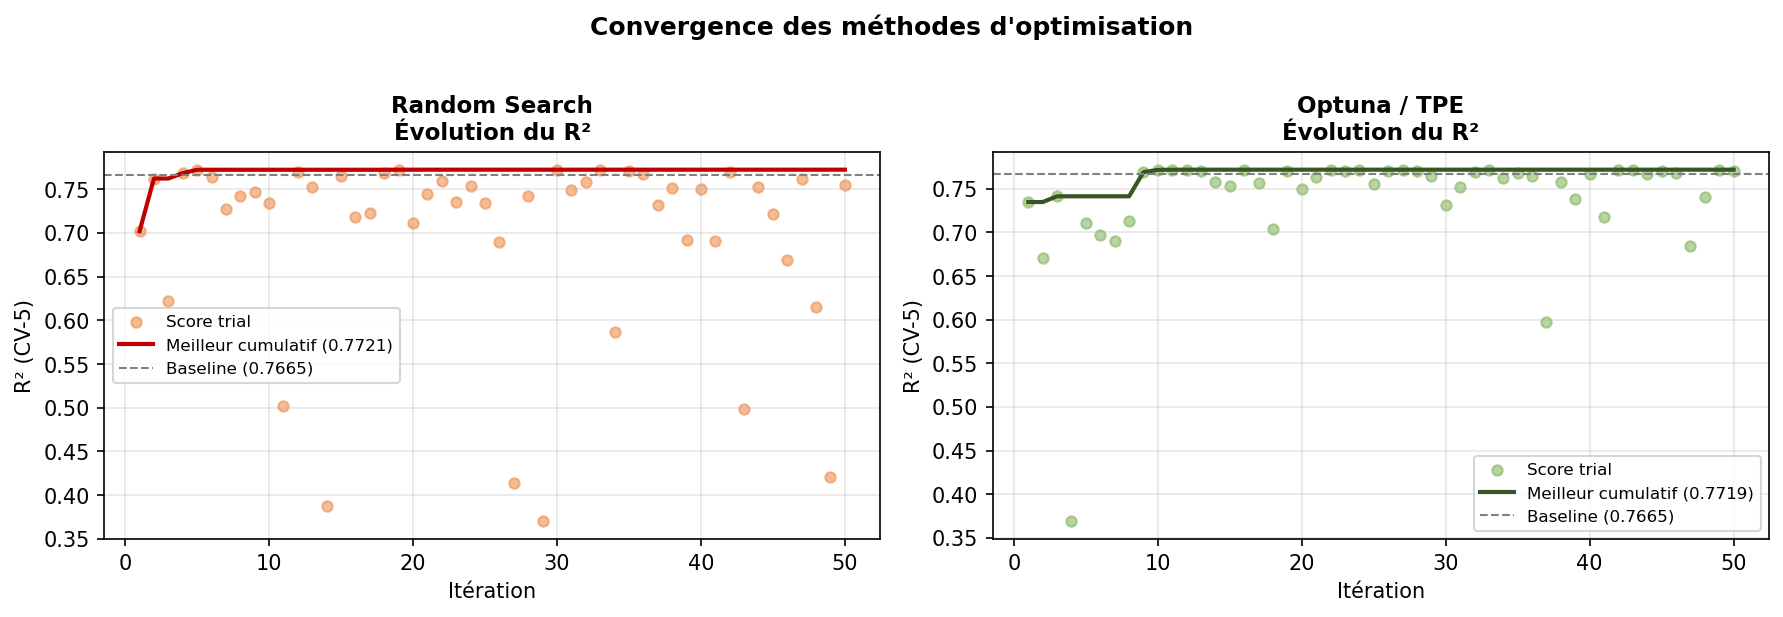
\includegraphics[width=\linewidth]{graph_evolution_r2.png}
  \caption{Évolution du $R^2$ cumulatif au fil des 50 itérations --
           Random Search (gauche) et Optuna/TPE (droite)
           \parencite{bergstra2012, akiba2019}. Optuna atteint son meilleur
           résultat dès les 10 premiers trials grâce au modèle surrogate
           TPE, tandis que Random Search converge plus progressivement.}
  \label{fig:evolution}
\end{figure}

\begin{figure}[H]
  \centering
  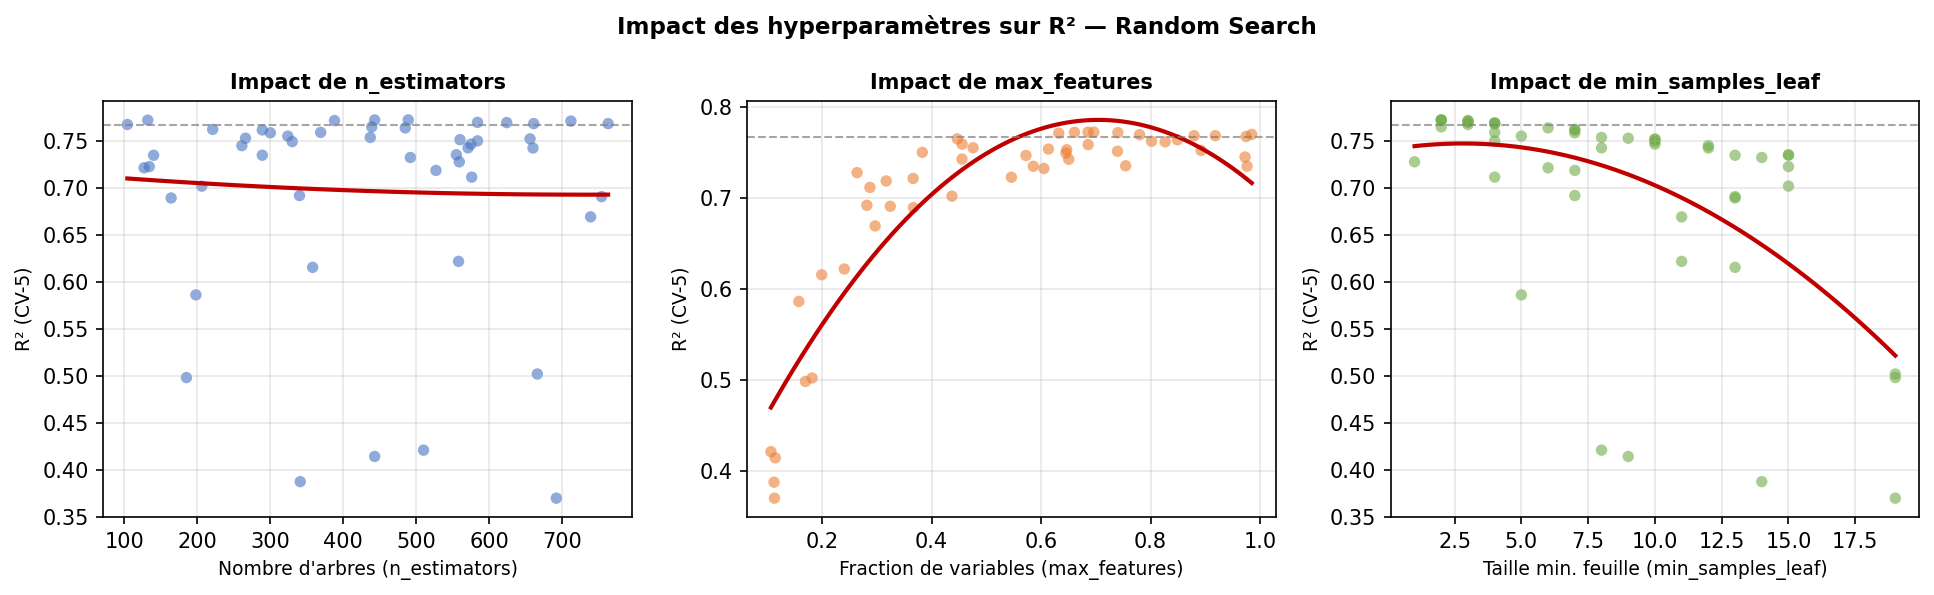
\includegraphics[width=\linewidth]{graph_impact_hyperparams.png}
  \caption{Impact de chaque hyperparamètre sur $R^2$ (Random Search).
           \code{max\_features} est de loin le paramètre le plus influent :
           les valeurs autour de 0.6--0.7 donnent systématiquement les
           meilleurs scores, confirmant l'analyse de
           \textcite{bergstra2012} sur la non-uniformité de l'influence
           des hyperparamètres.}
  \label{fig:hyperparams}
\end{figure}

\begin{figure}[H]
  \centering
  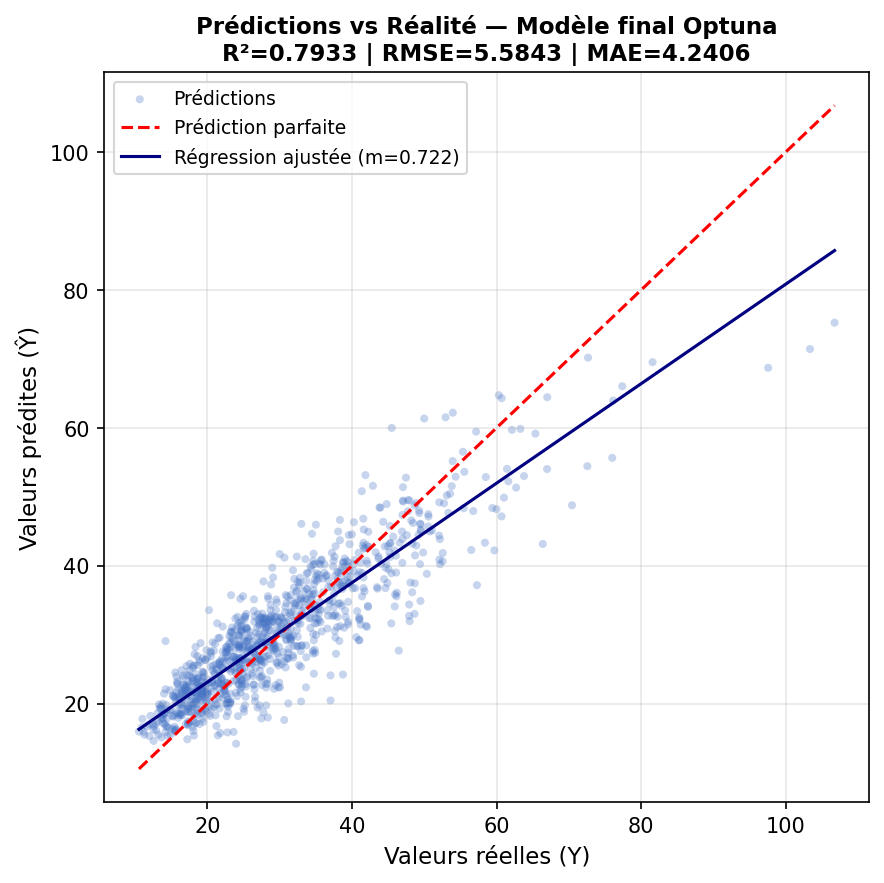
\includegraphics[width=0.70\linewidth]{graph_pred_vs_reel.png}
  \caption{Prédictions vs réalité -- modèle final Optuna/TPE
           \parencite{akiba2019} ($R^2=0.7933$, RMSE$=5.58$,
           MAE$=4.24$). Les points sont globalement alignés autour de la
           diagonale (prédiction parfaite en rouge). La pente de la
           régression ajustée ($m=0.722$) indique une légère
           sous-estimation pour les CLV élevées, attendue dans un
           contexte de valeurs hétérogènes.}
  \label{fig:predvsreel}
\end{figure}

%% ════════════════════════════════════════════════════════════
\section{Conclusion}
%% ════════════════════════════════════════════════════════════

Ce travail illustre l'apport conjugué de plusieurs leviers méthodologiques
pour améliorer la performance d'un modèle de classification multi-classes.

En Partie~A, la démarche itérative v1 $\to$ v9 a permis de progresser de
0.781 à \textbf{0.849 sur Kaggle Public (+8.7\,\%)}. Les gains les plus
significatifs proviennent : (i)~de l'architecture de stacking 3 niveaux
avec features originales dans le méta-modèle (+0.010 CV), fondée sur
\textcite{wolpert1992} et \textcite{breiman1996} ; (ii)~de l'intégration de
OvO GBM optimisé comme modèle de Niveau~1 \parencite{galar2011}, OvO
surpassant OvA de +0.062 en CV-5 isolé ; et (iii)~du seed averaging sur
5 seeds (+0.008 Kaggle), ancré dans les travaux d'\textcite{izmailov2018}
sur l'averaging stochastique et de \textcite{zhou2025} sur la variance
induite par le choix du seed. Le risque d'overfitting sur le Public LB a
été maîtrisé en conduisant toute l'optimisation sur le CV interne du train
set \parencite{bergstra2012}.

En Partie~B, les trois méthodes convergent vers des $R^2$ proches (0.769
à 0.772). Random Search \parencite{bergstra2012} et Optuna
\parencite{akiba2019} surpassent Grid Search \parencite{geron2019} en
identifiant des valeurs continues de \code{max\_features} ($\approx$
0.66-0.70) inaccessibles à une grille discrète. Le modèle final atteint
$R^2 = 0.793$ sur le jeu de test.

Ces résultats illustrent l'intérêt : (i)~d'explorer plusieurs familles de
modèles et décompositions binaires \parencite{galar2011} ; (ii)~d'investir
dans le feature engineering comportemental ; (iii)~d'utiliser des schémas
de validation OOF \parencite{wolpert1992} ; (iv)~de stabiliser les
prédictions par seed averaging \parencite{izmailov2018}.

\subsection*{Déclaration d'utilisation de l'IA générative}

Conformément aux directives du cours, nous déclarons avoir utilisé Claude
(Anthropic, \url{claude.ai}) pour : le débogage du code Python (stacking
OOF, notebook), les suggestions de structure du rapport, et la mise en
page du document. La méthodologie, le code, l'analyse et l'interprétation
sont notre travail original. Toutes les sources citées ont été vérifiées.

%% ════════════════════════════════════════════════════════════
\printbibliography[title={Références}]
%% ════════════════════════════════════════════════════════════

\end{document}
